\documentclass[a4paper, 11pt]{article}

\usepackage[left=2.5cm,right=2.5cm,top=3.5cm,bottom=3.5cm,bindingoffset=0cm]{geometry}

\usepackage[utf8]{inputenc}

\usepackage{float}
\usepackage{multirow}

\usepackage{graphicx}
\graphicspath{ {./} }

\usepackage[rightcaption]{sidecap}
\usepackage{hyperref}
\urlstyle{same}
\usepackage{fontawesome}
\usepackage{enumitem}
\usepackage{caption}


\usepackage{verbatim}

\usepackage{indentfirst}

\usepackage{lipsum}
\usepackage{booktabs}
\usepackage{tabu}
\usepackage[normalem]{ulem}

\usepackage{dblfloatfix}
\usepackage{placeins}


\renewcommand{\arraystretch}{1.5}

\usepackage{authblk}
\author[]{JSC "NEO Saint Petersburg Competence Center"}

\title{Public Version of the Research Plan for Distributed Decentralized Blockchain-based Storage Platform}

\begin{document}
\maketitle

\begin{abstract}

\textit{Distributed Decentralized Storage Platform} (DDSP) is a distributed 
decentralized object storage integrated with the Neo Blockchain. It is intended 
to be primarily used by Decentralized Applications (DApps) as a data storage 
and a Content Delivery Network (CDN). We propose using smart contracts to 
control the distribution of rewards from data owners and publishers between 
participants hosting data.

The first novelty of this research is approach based on homomorphic 
hash signatures to prove data integrity and availability to minimize 
load on the network and avoid transferring real data over the network in order to 
conduct data audit and validation. 

The second novelty is a scalable data placement method for \textit{DDSP}. Fine control 
over object location and minimal data movement in case of storage nodes 
failures are achieved by using a subset of a network map and storage 
policy rules for object placement and Rendezvous hashing for node selection.

\end{abstract}

\tableofcontents

\setlength{\parskip}{0.2cm}

\section{Motivation}

The development of blockchain technology has recently moved not so much
towards global public permissionless blockchains as towards the implementation
of corporate- and state use to solve specific internal tasks. It is logical
to expect the development of Dapp projects in this
direction. However, existing decentralized data storage solutions have not yet
been fully prepared to meet an emerging need for reliable, trusted data
storages with a secure and controlled integration of corporate- and public parts.

Currently, most projects in this field are aimed at implementing simple exclusive
storages of data of some users on capacities of other users or at creating
add-ons via IPFS for implementing public content distribution based on
traditional hosting and CDN. In this case, the niche of storages that have a
convenient API for DApp and the ability to organize isolated areas with control
over data exchange in both public- and other private data storage areas
is practically empty.

It is proposed to solve this problem relying on the Neo Blockchain mechanisms
as well as implementing novel approaches and technologies.

\textit{DDSP} is based on a peer-to-peer network that
use information from a smart contract and the Neo Blockchain to coordinate data
operations. X.509 PKI Neo Identity is planned to be applied to form isolated
storage networks and provide controlled access to data.

A storage network keeps information about its own topology with a
history of changes up to date and uses it when placing and searching for
data. The applied set of algorithms allows to minimize data movement
in the case of changing a network map, while ensuring the
specified storage policies.

\textit{DDSP} is aimed at ensuring data availability and
integrity. The integrity guarantee is achieved by using the proposed
novel data audit method, which is based on Homomorphic Hash functions, and
allows to verify the integrity of data on a storage node without sending real
data to a verifying party over a network. A computational complexity of
verifications depends linearly on the size of objects and is well suited for
parallelization. This approach not only reduces load on a network and storage
nodes but also allows to avoid data disclosure to a third party during a verification phase.

At a lower level, \textit{DDSP} provides backward
compatibility of a storage format with future versions of the system. This is
important not only for corporate use but also for DApp and smart contracts that
do not have a technical ability to modify codes or reallocate data in a network.

Thus, the proposed implementation of \textit{DDSP}
should ensure that the need of trusted data storages is met for both public use
and various private networks, while providing necessary guarantees of
information confidentiality, integrity and availability.

\section{System overview}

\begin{figure}[h]
\centering
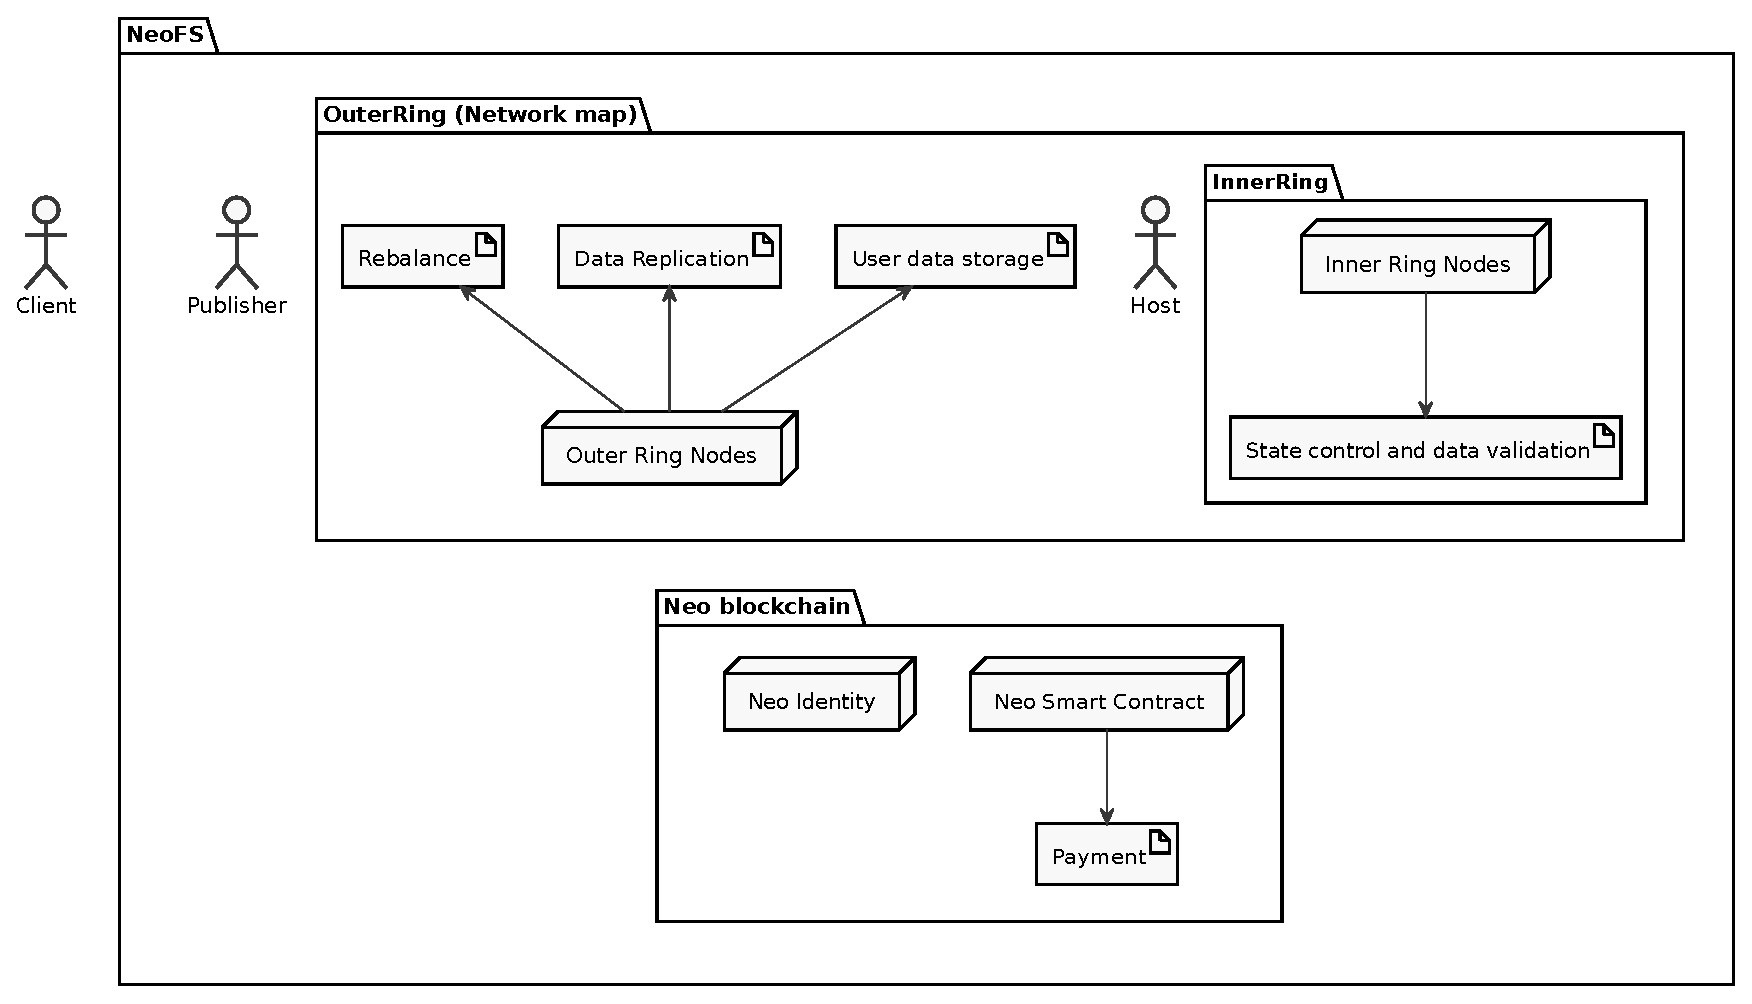
\includegraphics[scale=.55]{pic/overview1.eps}
\caption{System overview} 
\end{figure}

\subsection{Glossary}

\begin{itemize}[]
\item \textit{Network map} is a hierarchical structure in the form of a graph, describing available storage nodes

\item \textit{Epoch} is a time period during which a permanent network map exists

\item \textit{Homomorphic hash} is a hash resulting from applying homomorphic hashing to an object; it is used for zero-knowledge proof

\item \textit{Data audit} is data accessibility and storage validation process\end{itemize}

\subsection{Node Roles and Terms}

\begin{itemize}%[noitemsep]
        \item \textit{Inner Ring} -- network nodes executing a network state control and data validation
        \item \textit{Outer Ring} -- all other network nodes
\end{itemize}

Regardless of whether a node is in \textit{Inner} or \textit{Outer Ring}, it can perform one or more of the following roles:

\begin{itemize}[]

\item \textit{Host} is a computing system being a part of \textit{DDSP} and having at least the following features:
  \begin{itemize}%[noitemsep]
\item recent version of \textit{DDSP} software;
\item ID assigned by agreement with other nodes and unique within \textit{DDSP};
\item acceptable quality of communication channel with other \textit{DDSP} nodes;
\item storing and processing service/technical data of \textit{DDSP}, using its own capacity;
\item storing data according to parameters set by the system;
\item receiving and handling client queries according to the protocol/API used in \textit{DDSP}.

\end{itemize}

\item \textit{Publisher} is a computing system being a part of \textit{DDSP} 
  only in an incentive model, not being a part of a network map, related to a
  specific account of \textit{DDSP} (accounting) and
  interacting with the system via a specific protocol/API. \textit{Publisher} can
  get data from the system, place it for storing and receive responses to
  queries according to protocol/API used in \textit{DDSP}.
\item \textit{Client} is a computing system not being a part of
  \textit{DDSP}, interacting with the system via a
  specific protocol/API. \textit{Client} can receive data from the system, but can
  not place it for storing. It can also receive responses to queries according
  to protocol/API used in \textit{DDSP}.

\end{itemize}

\section{Network structure}

\textit{DDSP} is a p2p network which consists of
\textit{Inner} (nodes, specially selected by the network itself) and
\textit{Outer Rings} (all other network participants). Only nodes that provide
storage space for objects are included in the network map.

\textit{DDSP} is based on \textit{Inner Ring} nodes that
store information about the network state, metadata and state changes. In fact,
it is an append-only sharded database in the form of a distributed operations log
with signed snapshots at certain points in time.

For a consistent update of a distributed log, a consensus between nodes of
\textit{Inner Ring} is achieved using the dBFT protocol. A number of nodes
does not change during one epoch of the network map.
Nodes are admitted to \textit{Inner Ring} on the basis of X.509
certificates and signatures in the Neo Identity trust network or another X.509
PKI. The decision to remove a node from the ring is made based on its
inaccessibility or in case it is compromised. The usage of X.509 PKI allows to avoid
re-entering \textit{Inner Ring} by nodes with a poor reputation or unsatisfying
technical requirements.

Information from \textit{Inner Ring} is distributed to \textit{Outer Ring} via Gossip protocol.

\textit{Inner Ring} takes a decision on payments for storing data. A list of
\textit{Inner Ring} nodes is given in a smart contract. A candidate node from 
\textit{Outer Ring} nodes pays
a deposit that amounts to the cost of including/excluding a node in/from the list in
the smart contract to join queue for being added to \textit{Inner Ring}. 
When new nodes need to join \textit{Inner Ring} in order to
substitute non-available, discredited ones or increase a number of nodes to
support the network scalability, a node is selected from the ones being in the
queue. \textit{Inner Ring} nodes that have implemented correct data
validations and taken decisions on payments for data storing earn a low interest
on the paid amount.

\subsection{Bootstrapping} \textit{Inner Ring} nodes perform functions of
bootstrap nodes to initiate the work of \textit{Publisher}, \textit{Host} and \textit{Client} as well.
The bootstrap node returns a current state of event log (in general,
provides the procedure of retrieving a network map), therefore, providing nodes
and clients being connected with operations of storing and retrieving data. The
bootstrap node registers information on a \textit{Host} node to include it into a
network map of a succeeding epoch.

The bootstrap node may refuse a node registration or response.
Thus, it is important to know about all available nodes of \textit{Inner
 Ring}. A current list of \textit{Inner Ring} nodes can be achieved via a
smart contract call and is available on open resources.

\subsection{Network Map}

\textit{DDSP} keeps a network map up to date and 
distributes it over nodes. It contains information about groups of nodes, their
location in the network and main parameters necessary for correct data 
search and placement. The network map is a hierarchical structure that provides
available storage nodes. The network map is represented as a graph. The graph 
consists of vertices: buckets and nodes. A bucket is a vertex of the graph. 
Together with outbound edges, it forms a subgraph of the network map, leaves 
of which are represented by nodes. Nodes can only be leaves, the bucket can be 
a parent for other buckets or nodes. The bucket is characterized by type and value.

\subsection{Buckets}
In a decentralized system, it is impossible to fully control the correctness of
metadata provided by a storage node. Therefore, it is proposed to use
trustworthy buckets in a network map, i.e. the buckets that \textit{Inner Ring}
can form on its own, for example, ranking by GeoIP, AS, a confidence coefficient.
It is also assumed that a storage node can independently transmit information
about buckets in which it is located -- self-defined buckets. A user is
responsible for setting placement rules by using self-defined buckets.

\subsection{Distributed Log}

A distributed event log stores information about changes in the system state,
intermediate calculation data and other technical information necessary for
the operation of \textit{DDSP}. Each entry in the log is
consistent and signed by the nodes of \textit{Inner Ring}.

At epoch changes, a new network map (or difference with the previous version) is 
committed in the event log.

Each record in the log has a unique, monotonically increasing numeric
identifier. Periodically, the tail of the log is discarded and replaced with a
snapshot of the state.

Each node of a network records the last log position it knows and can
synchronize its state after loosing communication by reading all subsequent
blocks from the log. A new node, when it is connected to the network, needs to get
the most recent snapshot of the state.

\section{Data Placement}

\subsection{Placement Function and Placement Rule}

To get a subgraph of a network map or a subset of nodes where objects are
stored, the one needs to use a placement function that has the following
arguments:

\begin{itemize}%[noitemsep]
\item storage policy defined with a placement rule;
\item a network map (or a network map subgraph);
\item Rendezvous hashing salt.
\end{itemize}

A user can define a placement rule that is applied to a stored object. The
placement rule consists of a set of SELECT() or FILTER() operations applied to
a network map. The result of these operations is a subgraph of the network map
where data can be placed.

The SELECT() operation is applied to a tree. The operation inputs are a
replication factor at this level and a bucket type. Multiple operations in the
placement rule are put into order and each subsequent SELECT(r, type) operation
is applied to the result of the previous one.

The FILTER() operation is applied to a graph. The operation inputs are a
bucket type, a bucket value and a comparison operation. For text values, 
operations \textit{eq}, \textit{ne} are available. For numerical values,
\textit{gt}, \textit{ge}, \textit{lt} and \textit{le} are additionally
available.

A set of operations on the graph (in the placement rule) can be combined by
using AND, OR, NOT operations.

The placement function is executed recursively with the operation of the next
step being applied for all the nodes retrieved at the previous step. 

\begin{figure}[h]
\centering
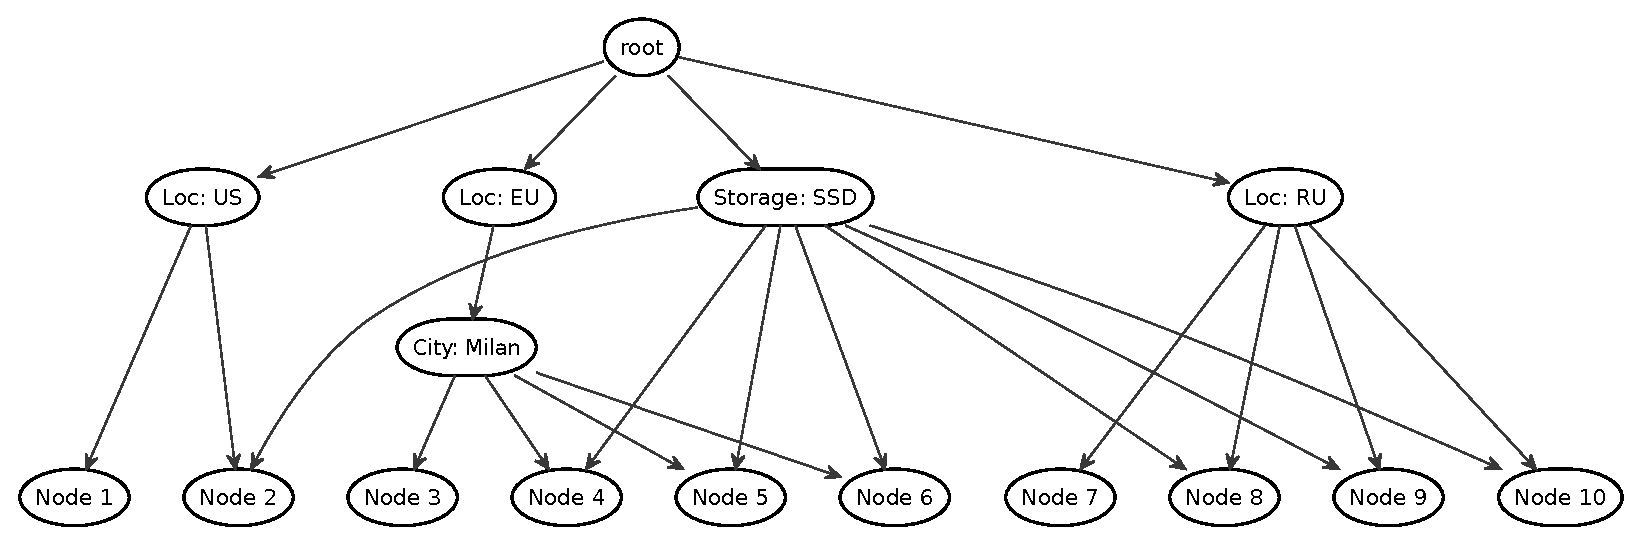
\includegraphics[scale=.62]{pic/uml_8_n_map_0.eps}
\caption{Network map example}
\end{figure}

This network map (or a network map subgarph) consists of the bucket with types Loc
(country), City (city), Storage (storage disk type) and the nodes of
corresponding buckets. The storage policy can be defined as follows:

\begin{itemize}%[noitemsep]
\item it is stored in 2 different countries;
\item it has 3 copies per each country;
\item it should be stored on SSD drives only.
\end{itemize}

This informal description should be represented as sets of SELECT(r, type) and
FILTER(type:value, op) operations. A total replication factor is obtained by
multiplying all the factors of each SELECT(r, type) replication. A final
statement should always be SELECT($ X $, Node).

\begin{table}[!h]

\begin{scriptsize}

\begin{tabular}{@{}|l|l|l|@{}}
\toprule
 Placement rule & Bucket result & Placement group result \\ \midrule

SELECT(2, Loc) & [ Eu ] $\cup$ [ Ru ] & \parbox{5.5cm}{[ [ Node 3, Node 4, Node 5, Node 6 ], [ Node 7, Node 8, Node 9, Node 10 ] ]}\\ \midrule

FILTER(Storage:SSD, equal) & \parbox{7cm}{( [ Eu ] $\cap$ [ Storage:SSD ] ) $\cup$  ( [ Ru ] $\cap$ [ Storage:SSD ] ) } & \parbox{5cm}{ [ [ Node 4, Node 5, Node 6 ], [ Node 7, Node 8, Node 9, Node 10 ] ]} \\ \midrule


SELECT(3, Node) & \parbox{7cm}{ ( $[N_1, N_2, N_3] \in $  ( [ EU ] $\cap$ [ Storage:SSD ] ) ) $\cup$  \\ (  $[N_4, N_5, N_6] \in $  ( [ Ru ] $\cap$ [ Storage:SSD ] ) ) } & \parbox{5 cm}{ [ [ Node 4, Node 5, Node 6 ], [ Node 8, Node 9, Node 10 ] ]} \\ \bottomrule

\end{tabular}
\end{scriptsize}

\caption{The placement rule application to the network map graph }
\end{table}

\begin{figure}[h]
\centering
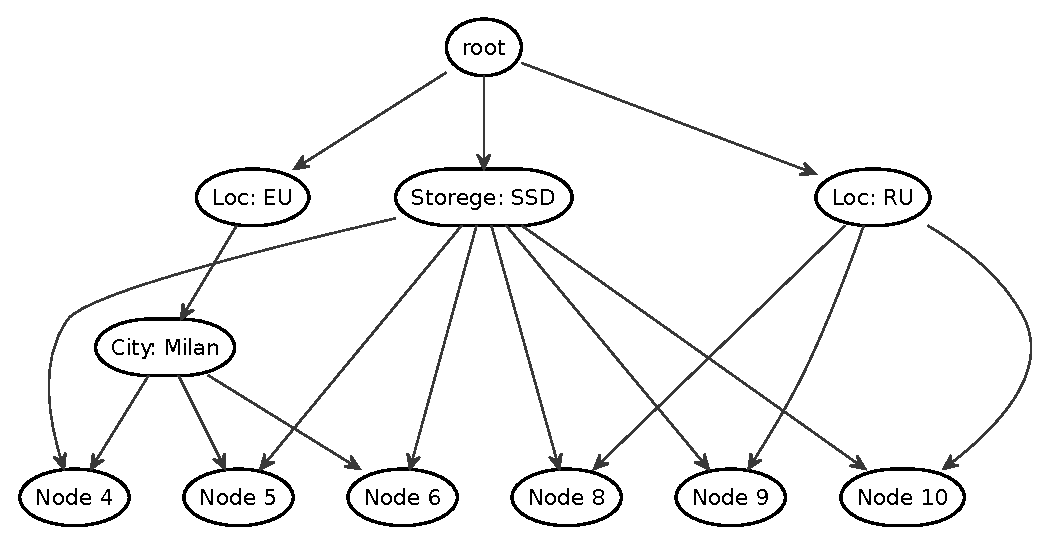
\includegraphics[scale=.62]{pic/uml_8_n_map_2.eps}
\caption{The obtained subgraph of the network}
\end{figure}

Thus, the subgraph of the network map and six nodes have been obtained, where
the object should be placed on to meet the placement policy requirements. The
result of the placement function operation is a subgraph of the network map --
\textit{Placement group} -- leaves of which are a deterministic and consistent list of
the storage nodes. If a storage policy, salt and a network map are known 
\textit{Placement group} can be retrieved without referring to a third party or storing
“object and storage node” pairs.

\subsubsection{Rendezvous Hashing}
Buckets and placement nodes in a bucket are selected using the Rendezvous hashing
algorithm. With it, each node or a bucket has an individual hash number for an
individual item, and the bucket or node, having the largest hash number, is chosen.
Data in this algorithm is distributed uniformly and a small number of data
movement is required when nodes are added or removed. However, it can achieve
minimum data movement when nodes are added or removed.

The basic idea is to give each node $N_j$ a score (weight) for each object
$O_i$, and assign the object to the highest scoring node. Firstly, all the clients
agree on a hash function h(). For object $O_i$, the node $N_j$ is defined to
have weight $w_{i,j}$ = h($O_i$, $N_j$). HRW assigns $O_i$ to the node $N_m$
whose weight $w_{i,m}$ is the largest. Since h() is agreed upon, each client can
independently compute the weights $w_{i,1}$, $w_{i,2}$, ..., $w_{i,n}$ and pick the
largest. If the goal is a distributed k-agreement, the clients can independently
pick the nodes with the k largest hash values.

If a node $N$ is added or removed, only the objects mapping to $N$ are remapped to
different nodes, satisfying the minimal disruption constraint above. The highest random weight
assignment can be computed independently by any client, since it depends only on
the identifiers for the set of nodes $N_1$, $N_2$, ..., $N_n$ and the object
being assigned.

\subsection{Container}
In order to place objects in the system a user needs to define a container.

The container has at least the following fields:
\begin{itemize}%[noitemsep]
\item an item uuid (for object addressing) being also salt required for a placement function to select buckets deterministically and pseudorandomly;
\item a container's owner;
\item a storage policy:
\begin{itemize}[noitemsep]
  \item a placement rule;
  \item a redundancy factor;\end{itemize}
\item a maximum capacity.
\end{itemize}The container defines the subgraph of a network map.

\subsubsection{Select Limitation and Container Registration}
The approach, where a complete network map, which includes all connected
nodes and plays the role of an initial graph, can impose additional costs when a
network expands. The allocation of limited space within the network map
(subgraph), called a container, allows to do the following:

\begin{itemize}%[noitemsep]
\item to isolate a subset of nodes. Handling the subset is faster and more
  predictable. After the container has been provided with a graph, container's
  network map traversal operations are faster;
\item to protect against overprovisioning -- the
  overall container`s capacity and its remaining capacity can be roughly estimated;
\item to control access to the container;
\item to simplify payment operations by linking them to the container;
\item to facilitate the integration of s3 and swift API for \textit{DDSP}.
\end{itemize}

To form a container`s subgraph, a replication factor in each SELECT(r, type)
call is increased by a redundancy factor $ K_r $. A container's uuid is
used as salt for selection in a placement function. An example, where $K_r=2$, is considered:

\begin{table}[!h]
\begin{scriptsize}
\begin{tabular}{@{}|l|l|l|l|@{}}
\toprule
Source & Placement rule & Placement function result & Salt              \\ \midrule
\multirow{2}{*}{Network Map} & SELECT($2 \cdot K_r$, Loc) & [ US , EU, RU, Ja ] & \multirow{2}{*}{Container salt} \\ \cmidrule(r){2-3}
 & SELECT($2 \cdot K_r$, node) & \parbox{6cm}{ [ [ $N_1$, $N_2$, $N_3$, $N_4$ ], [ $N_5$, $N_6$, $N_7$, $N_8$ ], [$N_9$, $N_{10}$, $N_{11}$, $N_{12}$], [ $N_{13}$, $N_{14}$, $N_{15}$, $N_{16}$] ] } &  \\ \bottomrule
\end{tabular}
\end{scriptsize}
\caption{Container}
\end{table}

As a result, a set of nodes that can be represented as a subgraph
of the network map is obtained. When forming the container, it is possible to
approximately estimate it's capacity. 

To do so, the weights of nodes are assigned depending on nodes' capacity. 
A total weight of the selected nodes has to correspond to the container's 
declared capacity. The object is placed into the container by using the 
placement function, where the hash of the object being placed is used as salt.

\begin{table}[!h]
\begin{scriptsize}
\begin{tabular}{@{}|l|l|l|l|@{}}
\toprule
Source & Placement Rule & Placement function Result & Salt              \\ \midrule
\multirow{2}{*}{Container} & SELECT(2, Loc) & [ US, Ja ] & \multirow{2}{*}{Hash of the object being placed} \\ \cmidrule(r){2-3}
 & SELECT(2, node) & [ [ $N_2$, $N_4$ ], [ $N_{15}$, $N_{16}$ ] ] &  \\ \bottomrule
\end{tabular}
\end{scriptsize}
\caption{Placement group}
\end{table}

\begin{figure}[!h]
\centering
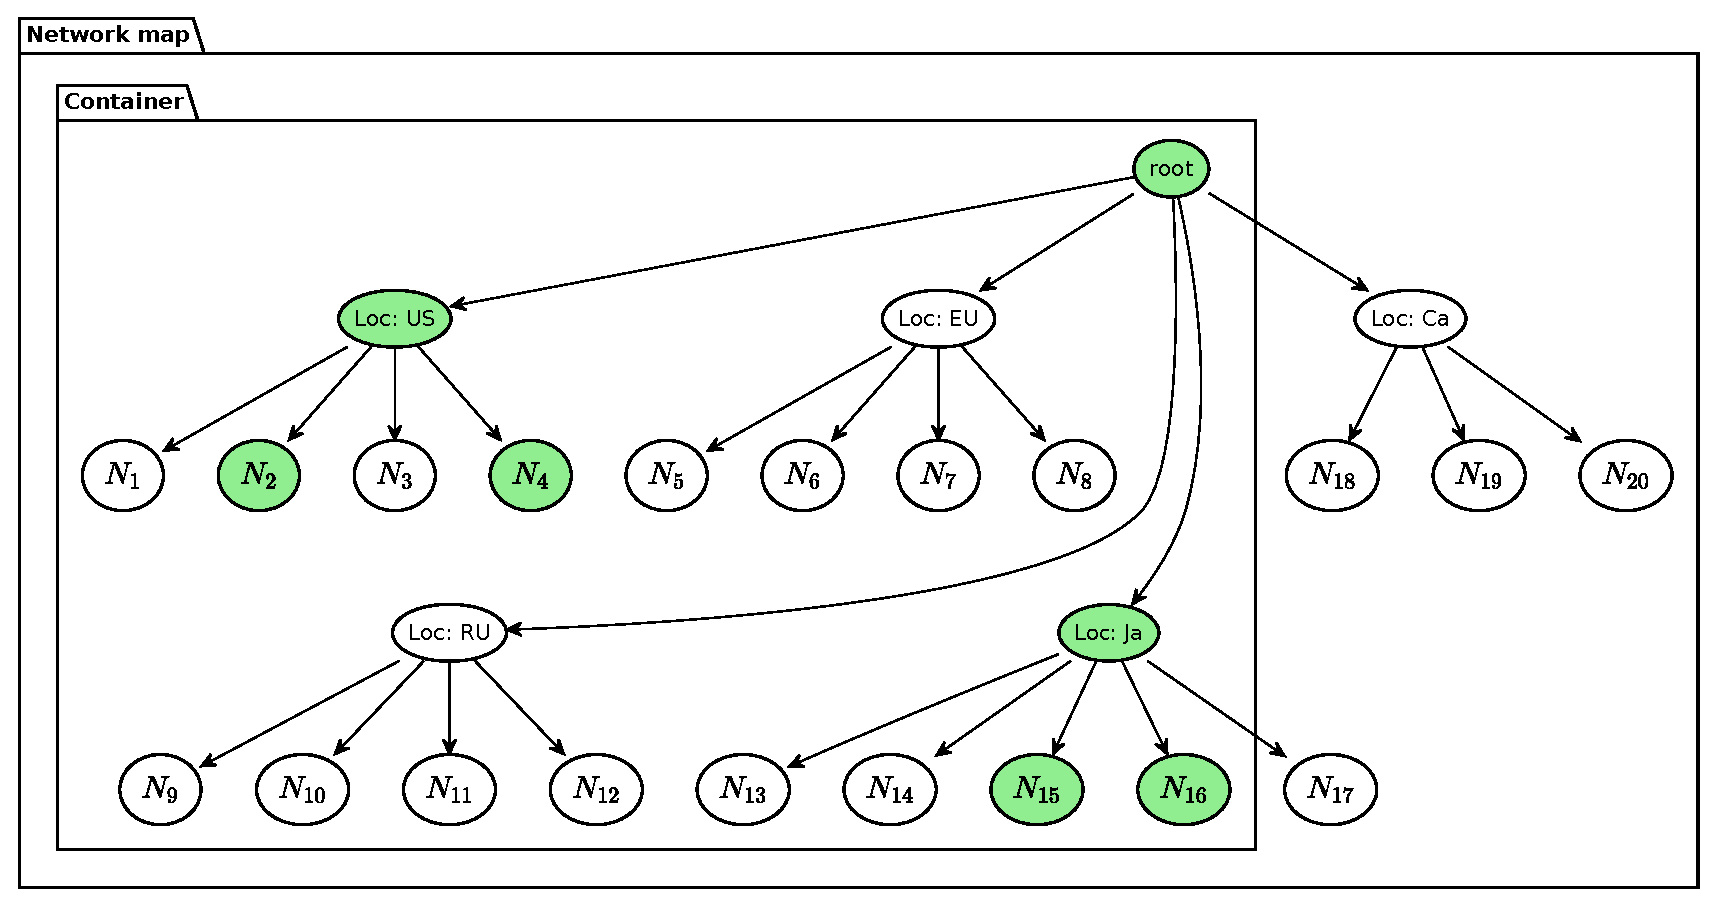
\includegraphics[scale=.55]{pic/uml_8_n_map_4.eps}
\centering
\caption{ An example of the placement function’s result}
\end{figure}

Highlighted buckets are \textit{Placement group} subgraph for the object.

\subsubsection{Matching Container Uuid and Storage Policy}

To encode a placement rule in a container uuid seems to be impossible since
the placement rule can be of an arbitrary complexity and length, with a set of
SELECT() and FILTER() operations for random buckets. A pair container's uuid -
placement rule needs to be stored and distributed in \textit{DDSP}. 
To match the container uuid and the placement rule, DHT is used.

Once the first query has been completed, the result is cached.

\section{Data Storage}

\subsection{Object Format}

To implement data storage and processing, the system operates with objects. An
object is a structure intended to be placed on a data storage device and
transmitted over a network. This structure consists of a user's data block of a
finite length and a set of headers containing information about the data and the
object itself. The size of the data in the object can be zero.

Firstly, there is a fixed header containing the version of the object format, its
total length, unique identifier, optional reference to a parent object,
electronic signature of a data publisher, type identifier of the
next extended header and identifier of the storage group.

The extended type header has a similar structure, and its last field indicates
the type of the next extended header. In this way, backward compatibility is
maintained at the data format level and the ability to extend supported functionality
is provided. In fact, the version of the data format is determined by the list of
known and supported formats of extended headers.

User data attached to the object is placed after headers.

The object in the system is immutable. It cannot be changed under any
circumstances.

\textit{DDSP} core works only with a fixed object
header and treats data as an immutable sequence of bytes without interacting
with the content.

Extended headers store information about user data properties, encryption
algorithms, checksum values, cryptographic signatures, identifiers, links to
other objects, etc. Extended headers are processed in the order of appearance by
separate data processing modules.

Such an object format allows, by delegating the processing and conversion of
user data to higher-level modules of the system, to organize complex schemes of
working with information.

At initial stages, to simplify the development, an object can be placed in a
file system of a storage node as a simple file. In the future, to improve the
performance and efficiency of using a disk subsystem, it is possible to directly use
raw block devices to store objects.

\subsection{Object Meta-Database}

Each node locally supports a meta-database of objects placed on it. The database
supports indexes for quick access to an object on a disk, graphs of links
between objects in a convenient representation, statistical information, and others
 necessary for the node to work.

The meta-database is an auxiliary database. It is neither replicated to other
nodes, nor stored in a blockchain. It can be completely restored based on
information from a network map, \textit{Inner Ring} and objects on a storage
node itself.

\subsection{N-factor Replication}

In the simplest storage policy case, a replication factor is set for an
object. During a control period, the object needs to be available in at least
a specified number of copies on different storage nodes.

\subsection{Erasure Coding}

When using erasure coding, data is divided into several parts so that the
original data can be restored even having an incomplete set of source parts. In
this case, a hierarchy of objects is created.

Information about the algorithm and parameters of erasure coding is placed in
the extended header of the root object.

\subsection{Availability and QoS/SLA}

A required level of object availability and parameters of service delivery are
a mater of finance and affect payments of rewards or assignment of penalties to
nodes.

The system can take into account the statistics of nodes when selecting
locations of a new object so that SLA requirements are highly likely to be met
in the future. However, this is a topic of further research.

\section{Data Audit}

In the decentralized storage system, where users no longer physically own the storage of their data, 
traditional cryptographic primitives for the purpose of data validation cannot be directly adopted. 
A group of works have been done focusing on attempt to solve a remote data validation task in a cloud 
storage.  These methods can be classified as Proof of Data Possession (PDP) and Proof of Retrievability (PoR). 

The PDP scheme initially has been presented by Ateniese et al. ("Provable Data Possession at Unstructured Stores", 2007). Related protocols detect a large amount of 
corruption in outsourced data. However, the schemes do not support the possibility to allow an external 
party to verify the correctness of remotely stored data without knowledge of data content, what is 
needed for decentralized storage systems. 

An efficient PDP method with privacy protection of users data from external auditors on a client and 
server sides is needed for a decentralized storage. From the perspective of data privacy protection, 
this drawback greatly affects the security of protocols. 

The design of \textit{DDSP} requires to develop an
efficient data validation method taking into account a network scalability issue, possibility to 
check data without knowledge of content and privacy protection of users data. 
It is proposed a zero-knowledge data validation method for a \textit{DDSP} for minimizing
data transferring to maintain a network scalability and minimizing a computational cost on the side
of a storage node to maintain a large number of parallel interactions, and on the side of a validating
node. The integrity guarantee is achieved due to the proposed data validation method based on the
homomorphic hash function which allows to verify the integrity of data on a storage node without
transferring real data to a validating party over the network. 

\subsection{Data Validation Method}

Requirements for the data validation method for \textit{DDSP}: 

\begin{itemize}
\item the ability to publicly verify stored data without an actual object ownership and the knowledge of an object content (zero-knowledge proof);
\item validation needs to ensure that a storage node’s response cannot be saved and repeated to counteract nodes-malefactors (method has to be developed in accordance with an arbitrary task of validation);
\item minimization of a computational cost on the side of a storage node to ensure a large number
of parallel interactions and on the side of a verifying node;
\item minimization of a network load to maintain a network scalability.
\end{itemize}

\subsubsection{Homomorphic Hashing}
In order to fulfill the requirements, the data validation method based on homomorphic hashing is proposed. 

A hash function has to have the following properties:
\begin{itemize}
\item it should be easily computable;
\item it should be computationally difficult to find collisions.
\end{itemize}

Homomorphic hash is a hash function that can compute a hash of a
composite block from hashes of individual blocks. 

A computational complexity of validations depends linearly on the size of validated data and is well suited for parallelization. 

In the proposed method, a challenge-response model is applied. 
In the simplest case, a request for an arbitrary set of hashes from the data being verified is considered.
The obtained hashes  have to produce an expected hash according to the rule of homomorphism. 

Validation of each individual object is a computationally expensive task for a decentralized system with an unlimited number of users and the amount of stored data. A storage group is introduced to reduce a computational cost and the amount of stored meta-information for validation. 

\subsubsection{Data Validation Complexity: Storage Group}

The concept of a storage group is introduced to reduce a validation complexity dependence
on the number of stored objects in the system. The storage group encapsulates a group of objects’
identifiers and a set of homomorphic hashes required for data validation. The safety and accessibility
of multiple objects in the network are achieved by the storage group validation without storing meta-information and conducting validation of each object. 
One container can have any number of storage groups. The storage group is located on the \textit{Inner Ring} nodes.
The storage group is an immutable structure, however, new storage groups can still be formed based on the 
existing ones (the merge operation) or the storage group can be removed (the objects will be deleted).
A group of homomorphic hashes is generated for data validation. A fixed number of hashes is created
from zones (first-level hashes).
A fixed and equal number of homomorphic hashes is stored for all the groups in \textit{DDSP}. 

In the simplest case, a validating node selects a
random first-level homomorphic hash during data validation and requests some number of second-level homomorphic hashes from  \textit{Placement group} nodes. 
Merging the second-level homomorphic hashes, a validating node confirms the validation if the obtained hash corresponds to the first-level hash being stored. 

\subsubsection{Challenge and Response}

Challenge is formed to confirm objects storage for the selected storage group. The division of nodes
into pairs, storing copies of one object, is formed to cover with a minimum combination of pairs of
nodes all nodes that store data from the selected verification area.

For each pair, a task is formed so that responses from one node can be checked by responses from
another one. As a challenge, the task is given to provide a certain number of homomorphic hashes from
a specific data range of the scanned object. The ranges in each case are determined pseudo-randomly so 
that a set of hashes of one node from the selected area of the object can be additionally checked by a
set of hashes from another node. At the same time, the object itself can be independently verified for
each node by hashing the responses received from it.

\subsubsection{Advantages}
The proposed method allows to minimize load on the network and validating nodes without
transferring a real data over the network. The storage group allows to keep a fixed amount of meta-information needed for validation process regardless of the size and the number of objects from the
storage group. 

\section{Data Replication}

Storage nodes have to control data replication since they are
motivated by incentive model to maintain an object storage policy in order
to get paid.

\subsection{Maintaining Storage Policy}
Storage nodes have to check the availability of a required
number of an object`s replicas that they store.

If the number of the object`s replicas is insufficient data is replicated to
maintain a storage policy. Data replication uses a placement function and
ignores failed nodes. This enables to deterministically define the nodes where
all network participants have replicated data. A container remains
consistent within one epoch (a single network map). An example for the policy:

\begin{scriptsize}
\indent SELECT(2, Loc) \\
\indent SELECT(2, node) \\
\indent $K_r$ = 2
\end{scriptsize}

\FloatBarrier

\begin{table}[!htbp]
\begin{scriptsize}
\begin{tabular}{@{}|l|l|l|@{}}
\multicolumn{2}{l}{}                           \\ \midrule
Placement rule & Placement function result            \\ \midrule
SELECT($2 \cdot K_r$, Loc) & [ US , EU, RU, Ja ] \\ \midrule
SELECT($2 \cdot K_r$, node) & \parbox{6cm}{ [ [ $N_1$, $N_2$, $N_3$, $N_4$ ], [ $N_5$, $N_6$, $N_7$, $N_8$ ], [$N_9$, $N_{10}$, $N_{11}$, $N_{12}$], [ $N_{13}$, $N_{14}$, $N_{15}$, $N_{16}$] ] } \\ \bottomrule
\end{tabular}
\end{scriptsize}
\caption{Container}
\end{table}
\FloatBarrier
 The object placement function have the following weight ratio:
\begin{scriptsize}

$w_{Loc:US} > w_{Loc:Ja} > w_{Loc:EU} > w_{Loc:RU}$

Loc:US: $w_{N_2} > w_{N_4} > w_{N_1} > w_{N_2}$

Loc:Ja: $w_{N_{16}} > w_{N_{15}} > w_{N_{14}} > w_{N_{13}}$

Loc:EU: $w_{N_{5}} > w_{N_{6}} > w_{N_{8}} > w_{N_{7}}$

\end{scriptsize}

\FloatBarrier

\begin{table}[!htbp]
\begin{scriptsize}
\begin{tabular}{@{}|l|l|l|@{}}
\multicolumn{2}{l}{}                           \\ \midrule
Placement rule & Placement function result            \\ \midrule
SELECT($2$, Loc) &  [ US, Ja ] \\ \midrule
SELECT($2$, node) & \parbox{6cm}{ [ [ $N_2$, $N_4$ ], [ $N_{15}$, $N_{16}$ ] ] } \\ \bottomrule
\end{tabular}
\end{scriptsize}
\caption{Placement group}
\end{table}

\FloatBarrier 

In the first case, let's consider the failure of the node $ N_ {16} $ in
the subgraph "Loc: Ja" where the subgraph can still follow the storage policy.
In this case, the verification node $ N_ {15} $ may mark the node $ N_ {16} $ as
the failed one and apply the placement function for the stored object, not
allowing for the node $ N_ {16} $ (Fig.5).

\FloatBarrier 

\begin{figure}[!h]
\centering
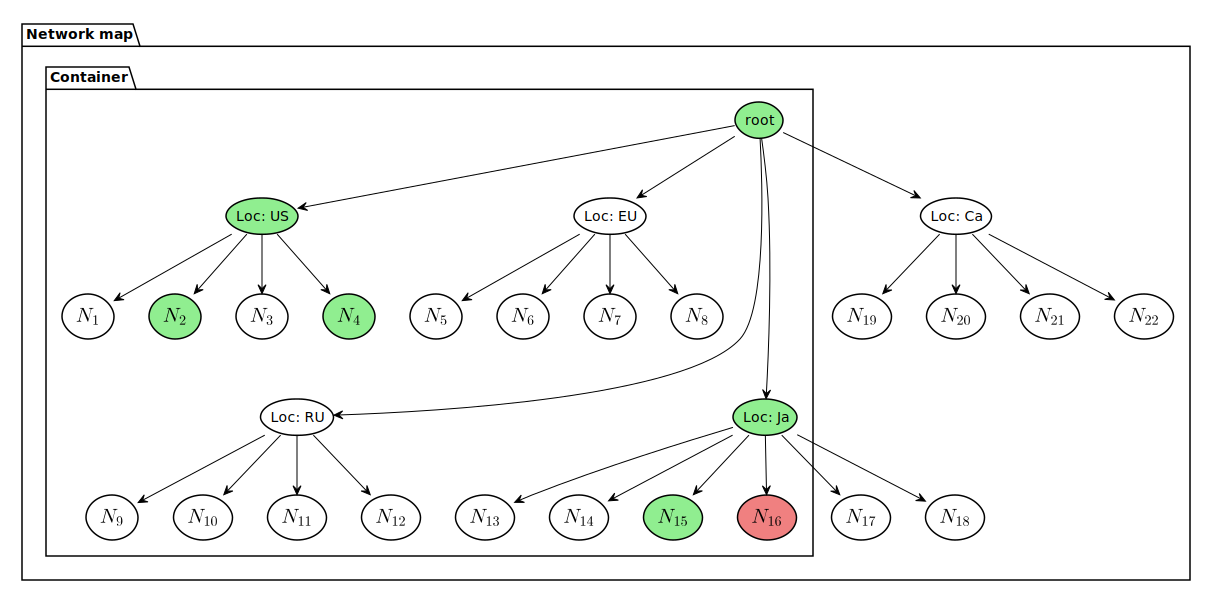
\includegraphics[scale=.5]{pic/uml_9_rebalance_1.eps}
\caption{ Example of the failed node }
\end{figure}

\FloatBarrier 

\FloatBarrier 

\begin{table}[!h]
\begin{scriptsize}
\begin{tabular}{@{}|l|l|l|@{}}
\multicolumn{2}{l}{}                           \\ \midrule
Placement rule & Placement function result            \\ \midrule
SELECT($2$, Loc) &  [ US, Ja ] \\ \midrule
SELECT($2$, node) & \parbox{6cm}{ [ [ $N_2$, $N_4$ ], [ $N_{14}$, $N_{15}$ ] ] } \\ \bottomrule
\end{tabular}
\end{scriptsize}
\caption{New Placement group}
\end{table}
\FloatBarrier 

The node $N_{14}$, having checked the node $N_{16}$ for unavailability, is
ready to receive a copy of the object from $N_{15}$ (Fig. 6).

\FloatBarrier 

\begin{figure}[!h]
\centering
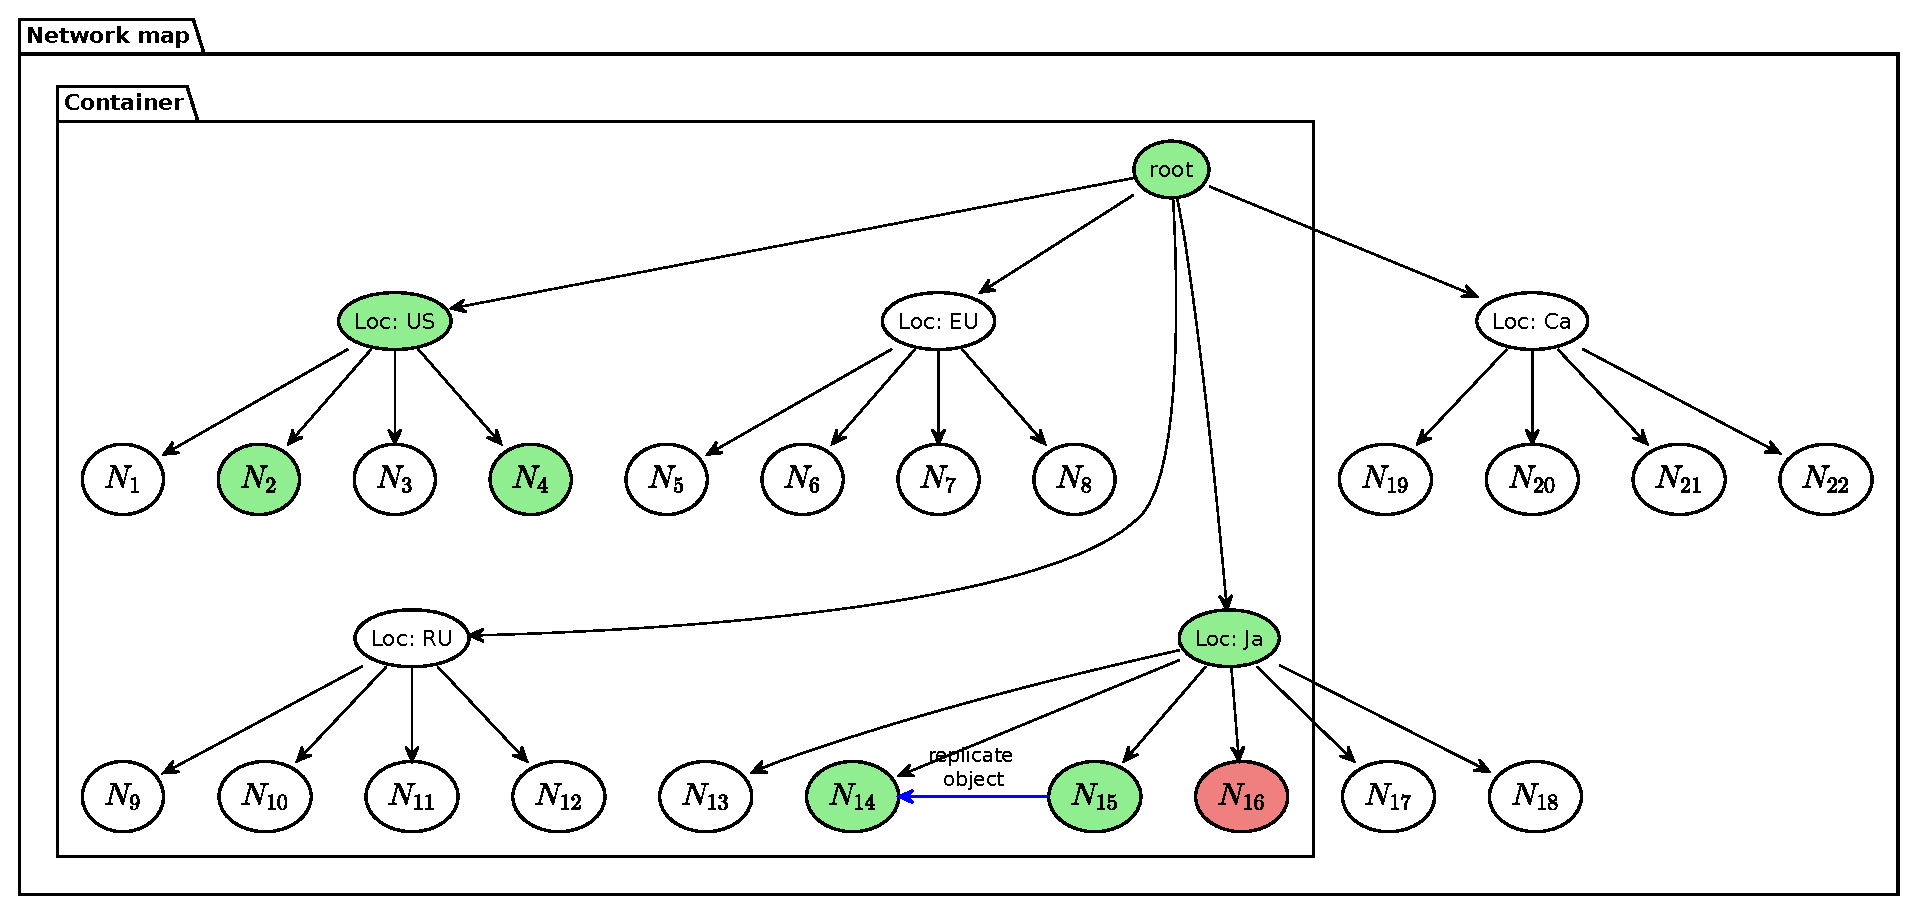
\includegraphics[scale=.5]{pic/uml_9_rebalance_2.eps}
\caption{ Object replication }
\end{figure}

\FloatBarrier 

The case, where the subgraph can not follow the storage policy due to
the failure of several nodes ($N_{13}$, $N_{15}$, $N_{16}$), is considered (Fig. 7).

\FloatBarrier 
\begin{figure}[!h]
\centering
\includegraphics[scale=.5]{pic/uml_9_rebalance_3.eps}
\caption{ Example of the failed nodes }
\end{figure}
\FloatBarrier 

In this case, the nodes are marked as failed and the object placement function
is applied. Instead of the subgraph "Loc: Ja" that does not meet the
storage policy now, the object placement function chooses the next by weight
subgraph that does meet the requirements of the storage policy -- "Loc: EU".
According to Rendezvous hashing by maximum weights, the nodes $N_5$ and $N_6$
are selected for placement (Fig. 8).

\FloatBarrier 

\begin{table}[!htbp]
\begin{scriptsize}
\begin{tabular}{@{}|l|l|l|@{}}
\multicolumn{2}{l}{}                           \\ \midrule
Placement rule & Placement function result            \\ \midrule
SELECT($2$, Loc) &  [ US, EU ] \\ \midrule
SELECT($2$, node) & \parbox{6cm}{ [ [ $N_2$, $N_4$ ], [ $N_{5}$, $N_{6}$ ] ] } \\ \bottomrule
\end{tabular}
\end{scriptsize}
\caption{Placement group}
\end{table}
\FloatBarrier 

\begin{figure}[!h]
\centering
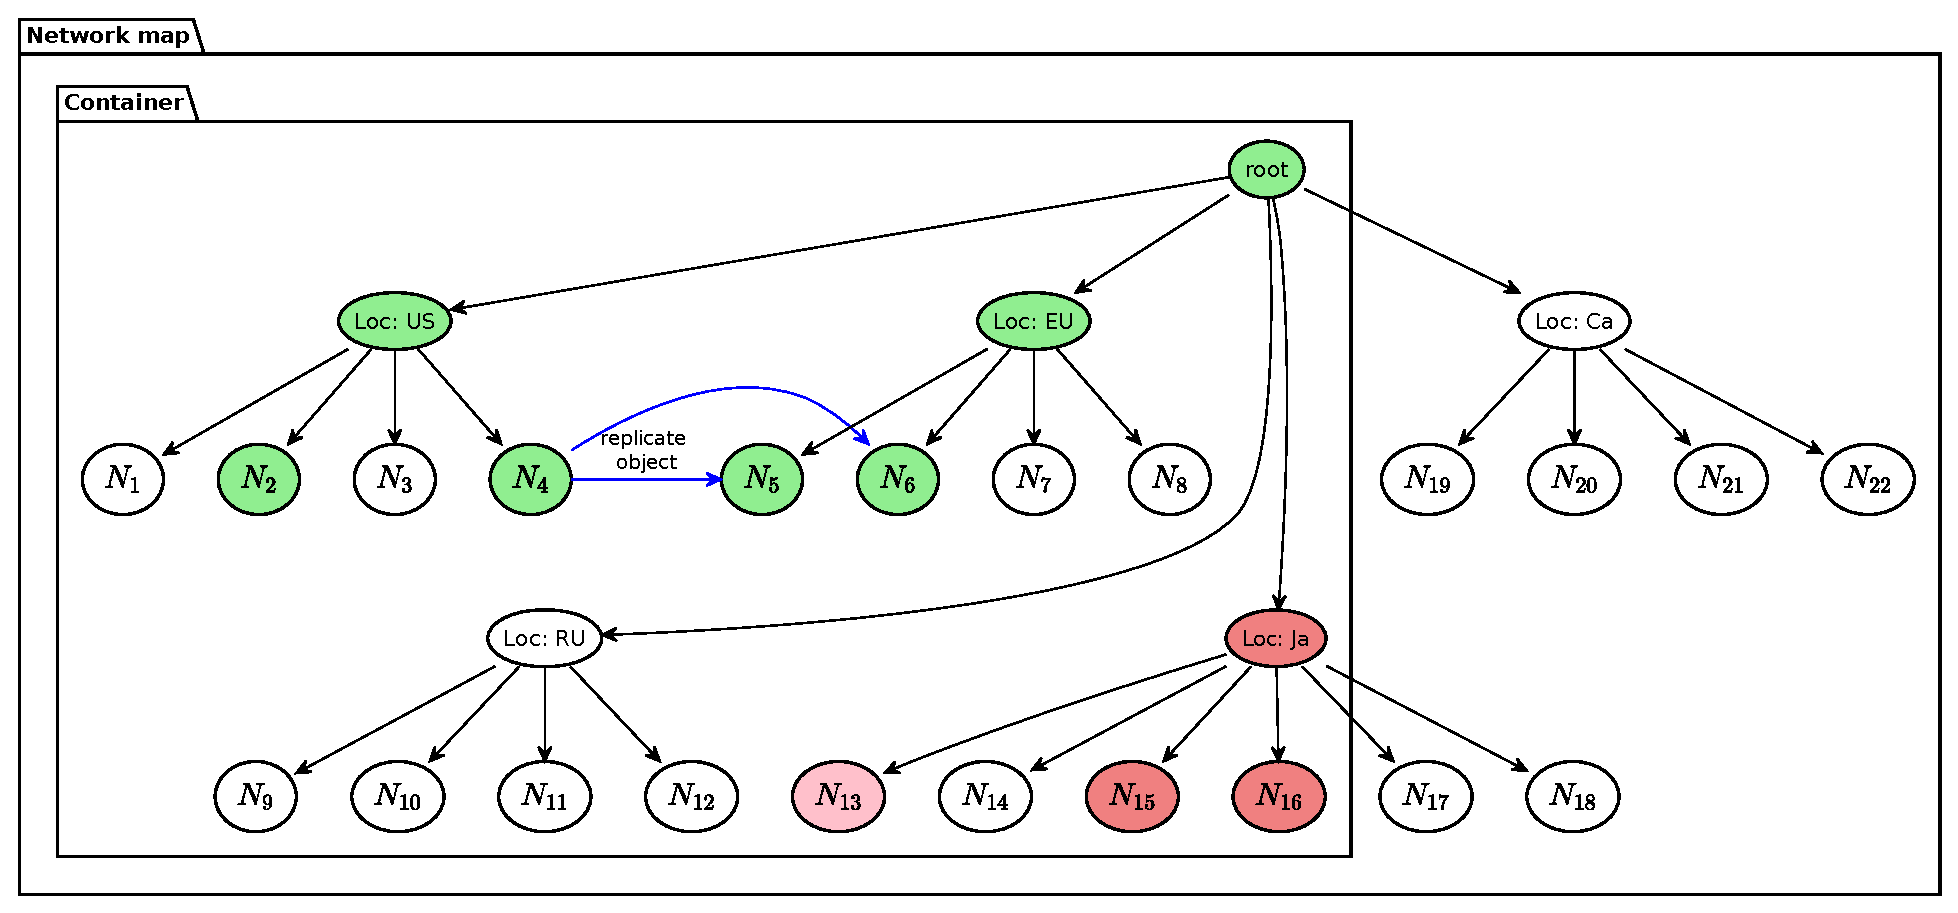
\includegraphics[scale=.5]{pic/uml_9_rebalance_4.eps}
\caption{ Object replication }
\end{figure}

\FloatBarrier 

\subsection{Reorganization and Data Movement }

When changing an epoch, a situation may arise where data needs to be
rebalanced, if a node storing an object no longer falls into a placement
group. In this case, it checks that the object is available in a new storage
group; afterwards the object can be deleted.

\section{Data Services}
\subsection{End-to-end Encryption}

The core of the system does not deal directly with user data, so a data
publisher is responsible for data encryption. To save information about
encryption keys, algorithms and signatures, the corresponding extended object
headers are used. Control of encryption keys is assigned to the data publisher.

\subsection{Data Deduplication}

Through the mechanism of representing an object, which consists of references
to data from other objects, data deduplication can be
implemented at a block level using the algorithm for reconciling the hashes
of data with a sliding window when uploading data into the system.

\subsection{POSIX-like FS}

Representing \textit{DDSP} as a fully POSIX-compatible
file system is a challenge because of differences in data models. At the first
stage, it is suggested implementing access in the ``read-only mode'', with only
regular files and directories supported.

From the previous experience, this should already be enough for integration with
most legacy applications.

The implementation of access support with the possibility of writing requires
further research.

\subsection{HTTP Gateway}

It seems favourable to develop a module for Nginx that implements an internal
data access protocol, for support in HTTP. At the first stage, it is suggested
implementing access in the ``read-only mode'' only.

\subsection{External Storage Integration}

To efficiently adopt \textit{DDSP} in existing projects,
it is necessary to have a possibility to use existing data storage systems. The
most popular protocols that need to be supported are AWS S3 and OpenStack Swift.

For data in an external system, it is suggested creating objects with a null
data block and an extended header that contains the address of an object in the
external system.

\section{Neo Blockchain}

\subsection{Distributed Decentralized Storage Platform PKI}

If X509 PKI is used, a node authentication for connecting to a network has to be
done together with verifying the node certificate signature. In the absence of
an external Certification Authority (CA) and the mechanism for issuing and
distributing certificates, it makes sense to develop CA integrated with NeoID
and used Automated Certificate Management Environment (ACME) protocol for
issuing certificates. As a \textit{Client} Challenge, the proof of ownership of NeoID can
be used.

\subsection{Neo Ecosystem}

As a common solution, \textit{DDSP} is integrated
as an element of Neo Ecosystem with a deposit-based payment by the GAS tokens and 
is based on the Neo smart contract. 

We are considering different options for using \textit{DDSP}: as an ecosystem element for 
internal and external use in the NEO blockchain, and integration with other projects.

External use:
\begin{itemize}
\item user data storage;
\item neo blockchain-based DApps can use the storage for keeping data;
\item storing data and files for smart contracts.
\end{itemize}

Possible Neo blockchain internal use:
\begin{itemize}
\item Storing smart contract code with keeping only the hash of the smart contract script in the blockchain to reduce a deployment cost;
\item Old Block Data can be stored by the storage, not by Full Nodes as it now, to increase the Neo blockchain scalability.
\end{itemize}

Neo smart contract is used as a
deposit storage of the \textit{Publisher}'s payment for subsequent phased
distribution between storage nodes after verification of initiated data
availability (data audit). 

In addition, smart contract saves a list of nodes to enter \textit{Inner
  Ring} and an updated list of \textit{Inner Ring} nodes as well as information
for their identification.

\subsection{Neo Smart Contract: Payments and Accounting}

Accounting is based on the Neo Blockchain. Primary asset storage in \textit{DDSP} is a
smart contract. We deploy the smart contract into the NEO Blockchain and expose it as a
wallet address. \textit{DDSP} users might transfer assets to this wallet, what is equal
to deposit placement into the system.

\textit{Inner Ring} nodes run a blockchain explorer in the background and monitor assets
movement to the smart contract wallet. Through transaction details analysis, we
can define the sender's wallet as a ScriptHash and use it as an identity in the system. Users' deposits are stored in local databases and are synchronized among
nodes via consensus.

The smart contract provides a call to the user to withdraw assets from the deposit back
to his wallet. This call costs a small amount of GAS and is stored in
the blockchain as a transaction. A once written transaction is noted by 
blockchain monitors, and a selected \textit{Inner Ring} node by the consensus sends the transaction for
assets transfer from the smart contract wallet to the user's one.

Besides payments routine, the smart contract is used as a key storage. We store
two things: \textit{Inner Ring} nodes public keys and \textit{Inner Ring} entrants queue.

\textit{Inner Ring} keys storage lets verify the initiator of the smart contract calls related to transfer of rewards
through the 'CheckWitness' syscall. Thus, an \textit{Inner Ring} node can only initiate payouts to \textit{Hosts}.

When \textit{Host} is going to become an \textit{Inner Ring} node, it should place enough deposit
and put itself into the entrants queue. This requires a certain amount of GAS to call the smart contract. The payment confirms the intention of \textit{Host} to serve administrative tasks of \textit{DDSP}.

The placed deposit is considered as an advance payment for(1) the smart
contact call to remove \textit{Host} from the queue, (2) the smart contact call to add a \textit{Host}'s key
to \textit{Inner Ring} keys list and (3) the smart contract call to remove it from the list, upon
\textit{Host} requests to leave \textit{Inner Ring}.

\section{A View to the Future}
\begin{itemize}
    \item The possibility of paying in fiat- and crypto-currency (\textit{nash.io} can be
      used to convert input payments into GAS) to be considered

    \item The HTTP access to stored objects (gates) for public data to be
      implemented

    \item Integration with other Neo Ecosystem projects to be provided

    \item The possibility of storing Old Block Data instead of Full Nodes by
      \textit{DDSP}, to increase the Neo blockchain
      scalability, to be studied

    \item The possibility of creating private payment channels

\end{itemize}

\vspace{2mm}

\section{Incentive Model}

\begin{itemize}
    \item It is necessary to solve the problem with latency and bandwidth
      overhead associated with the use of the platform

    \item It is necessary to ensure the storage cost is lower than existing
      solutions, such as Amazon S3, Microsoft Azure and others. At the same
      time, it is necessary to set a sufficient storage cost to enable storage
      nodes to make profit
\end{itemize}

Possible ways of commercializing the project:
\begin{itemize}
  \item get royalty from successful smart contract operations;
  \item build a group of own storages to share storage capacity;
  \item adapt the project to private storage solutions, for different business customers.
\end{itemize}

\vspace{2mm}

\vspace{10mm}

\section{Distributed Decentralized Storage Platform Advantages}

\begin{itemize}
    \item A unique data audit method that has a minimum load on the network
      and a computing power of verifying- and verified parties

    \item Building a p2p network by using a unique data placement method
      reduces the network load

    \item Truly decentralized without a single point of failure

    \item \textit{DDSP} versioning support

    \item Support for private- (encrypted) and public data

    \item Optional support for erasure codes

    \item Platform that can be used in various Dapps for the Neo Blockchain

    \item API S3 and Swift compatibility

    \item The system works with both a normal disk space and private data
      storage space that works with various protocols (Swift / s3 and etc)

    \item Private storage can be implemented on \textit{DDSP} for specialized business tasks

\end{itemize}

\vspace{2mm}

\section{Points to Research}

\begin{itemize}

    \item Options for the execution of data audit procedures using homomorphic
      hashes

    \item Using of node statistics when selecting a node to store an object to
      ensure the required probability of object availability

    \item Algorithm to calculate an optimal number of copies of each object
      based on a minimum cost of data storage with requested storage policy

    \item It is necessary to consider the possibility of supporting popular
      protocols AWS S3 and OpenStack Swift for storing objects in the existing
      storage node of traditional systems, the space of which can be used for
      \textit{DDSP}

    \item Methods to increase data availability (erasure coding optimized for
     \textit{DDSP} or other algorithms)

    \item Metadata format and object header fields

    \item Search for the optimum implementation of meta-databases

    \item Possibility of using private channels to pay for object storage

    \item Variants of a smart contract work logic and payment model for object
      storage

    \item Incentive model and Economic Research

\end{itemize}

%\vspace{20mm}

\hspace*{-3.4cm}

\end{document}
